\documentclass[utf8,usehyperref,12pt]{G7-32}
\usepackage[T2A]{fontenc}
\usepackage[utf8]{inputenc} %% ваша любимая кодировка здесь
\usepackage[russian]{babel} %% это необходимо для включения переносов
\usepackage{float}
\usepackage{textcase} 
\usepackage{lastpage}
\usepackage[dvips]{graphicx}
\graphicspath{{pictures/}}
\DeclareGraphicsRule{*}{eps}{*}{}
\TableInChaper % таблицы будут нумероваться в пределах раздела
\PicInChaper   % рисунки будут нумероваться в пределах раздела
\setlength\GostItemGap{2mm}% для красоты можно менять от~0мм

% Определяем заголовки для титульной страницы
\NirOrgLongName{
Министерство общего и профессионального образования РФ

\MakeUppercase{Санкт-петербургский государственный университет информационных технологий, механики и оптики}
}
%\NirBoss{Научный руководитель}{И.И.Упырёв} %% Заказчик, утверждающийНИР
\NirManager{Научный руководитель}{Р.~В.~Иванов} 

\NirYear{2010}%% если нужно поменять год отчёта; если закомментировано, ставитсятекущий год
\NirTown{г. Санкт-Петербург,} %% город, в котором написан отчёт
% по проекту \No8550: 

% \NirIsAnnotacion{АННОТАЦИОННЫЙ } %% Раскомментируйте, если это аннотационный
%отчёт

\NirUdk{УДК \No 2123132123}
\NirGosNo{Регистрационный \No 123123}

%\NirStage{Этап \No 1.1}{промежуточный}{<<Обзор современного состояния торсионных
%наногенераторов>>} %%% Этап НИР: {номер этапа}{вид отчёта - промежуточный или
%заключительный}{название этапа}

\bibliographystyle{unsrt} %Стиль библиографических ссылок БибТеХа

%%%%%%%<------------- НАЧАЛО ДОКУМЕНТА
\begin{document}
\usefont{T2A}{ftm}{m}{} %%% Использование шрифтов Т2 для возможности скопировать
%текст из PDF-файлов.

\frontmatter %%% <-- это выключает нумерацию ВСЕГО; здесь начинаются
%ненумерованные главы типа Исполнители, Обозначения и~прочее

\NirTitle{\textbf{<<Выпускная квалификационная работа>>}}
%%% Название НИР и~генерация титульного листа


\Executors %% Список исполнителей здесь
%% это рисует линию размера 3мм и~толщиной 0.1 пункт
\begin{longtable}{p{0.35\linewidth}p{0.2\linewidth}p{0.35\linewidth}}
Научный руководитель, 	&		&	\\
Р.В.~Иванов	&\rule{1\linewidth}{0.1pt}	&  \\ \vspace{1cm}

Выполнил  &		&	\\
Н.В.~Назаренко, & \rule{1\linewidth}{0.1pt}& \\
\end{longtable}

\Referat %% Реферат отчёта, не~более 1 страницы
Отчёт \pageref{LastPage}~c. 4~рис., 3~табл.

\MakeUppercase{Linux, хранилилище, webdav}



\tableofcontents

%\NormRefs % Нормативные ссылки 
%\Defines % Необходимые определения 



\Introduction

placeholder

\mainmatter %% это включает нумерацию глав и~секций в документе ниже

\chapter{Глава 1. Обзор и техническое задание}

\section{Обзор особенностей заказчика}
\subsection{Организационная структура}
Санкт-петербургский городской дворец творчества юных обладает большой и сложной организационной структурой, для каждого 
элемента которого, характерен свой вид деятельности. Рассмотрим организацию с точки зрения двух аспектов: территориального
и структурного.

Территориальная распределенность обусловленна тем, что Дворц творчества юных расположен в центре города, на его территории находиться множество отдельных корпусов, а также ему принадлежит довольно большой участок земли на Крестовском острове и ЗЦДЮТ «Зеркальный». Доступ пользователей к глобальным и локальным информационным ресурсам обеспечивается подключениями по выделенной линии
(2 мб/с), по оптоволокну (1000 мб/с) и прямыми подключениями к узлу (100 мб/с). Сеть рассчитана на большое количество пользователей ИТ-инфраструктурой (более
15 000 компьютеров). Среди них: работники дворца; педагоги; управляющий персонал;  персонал, отвечающий за сервисную деятельность; учащиеся. Сложность управленческой структуры организации определяется большим штатом сотрудников и широким спектром исполняемых функций. Главным руководителем является генеральный директор, которому подчиняются различные подразделения такие как: финансовый, хозяйственный, учебно-воспитательный и другие сектора.

\begin{figure}[ht]
   \centering%центрируем картинку
   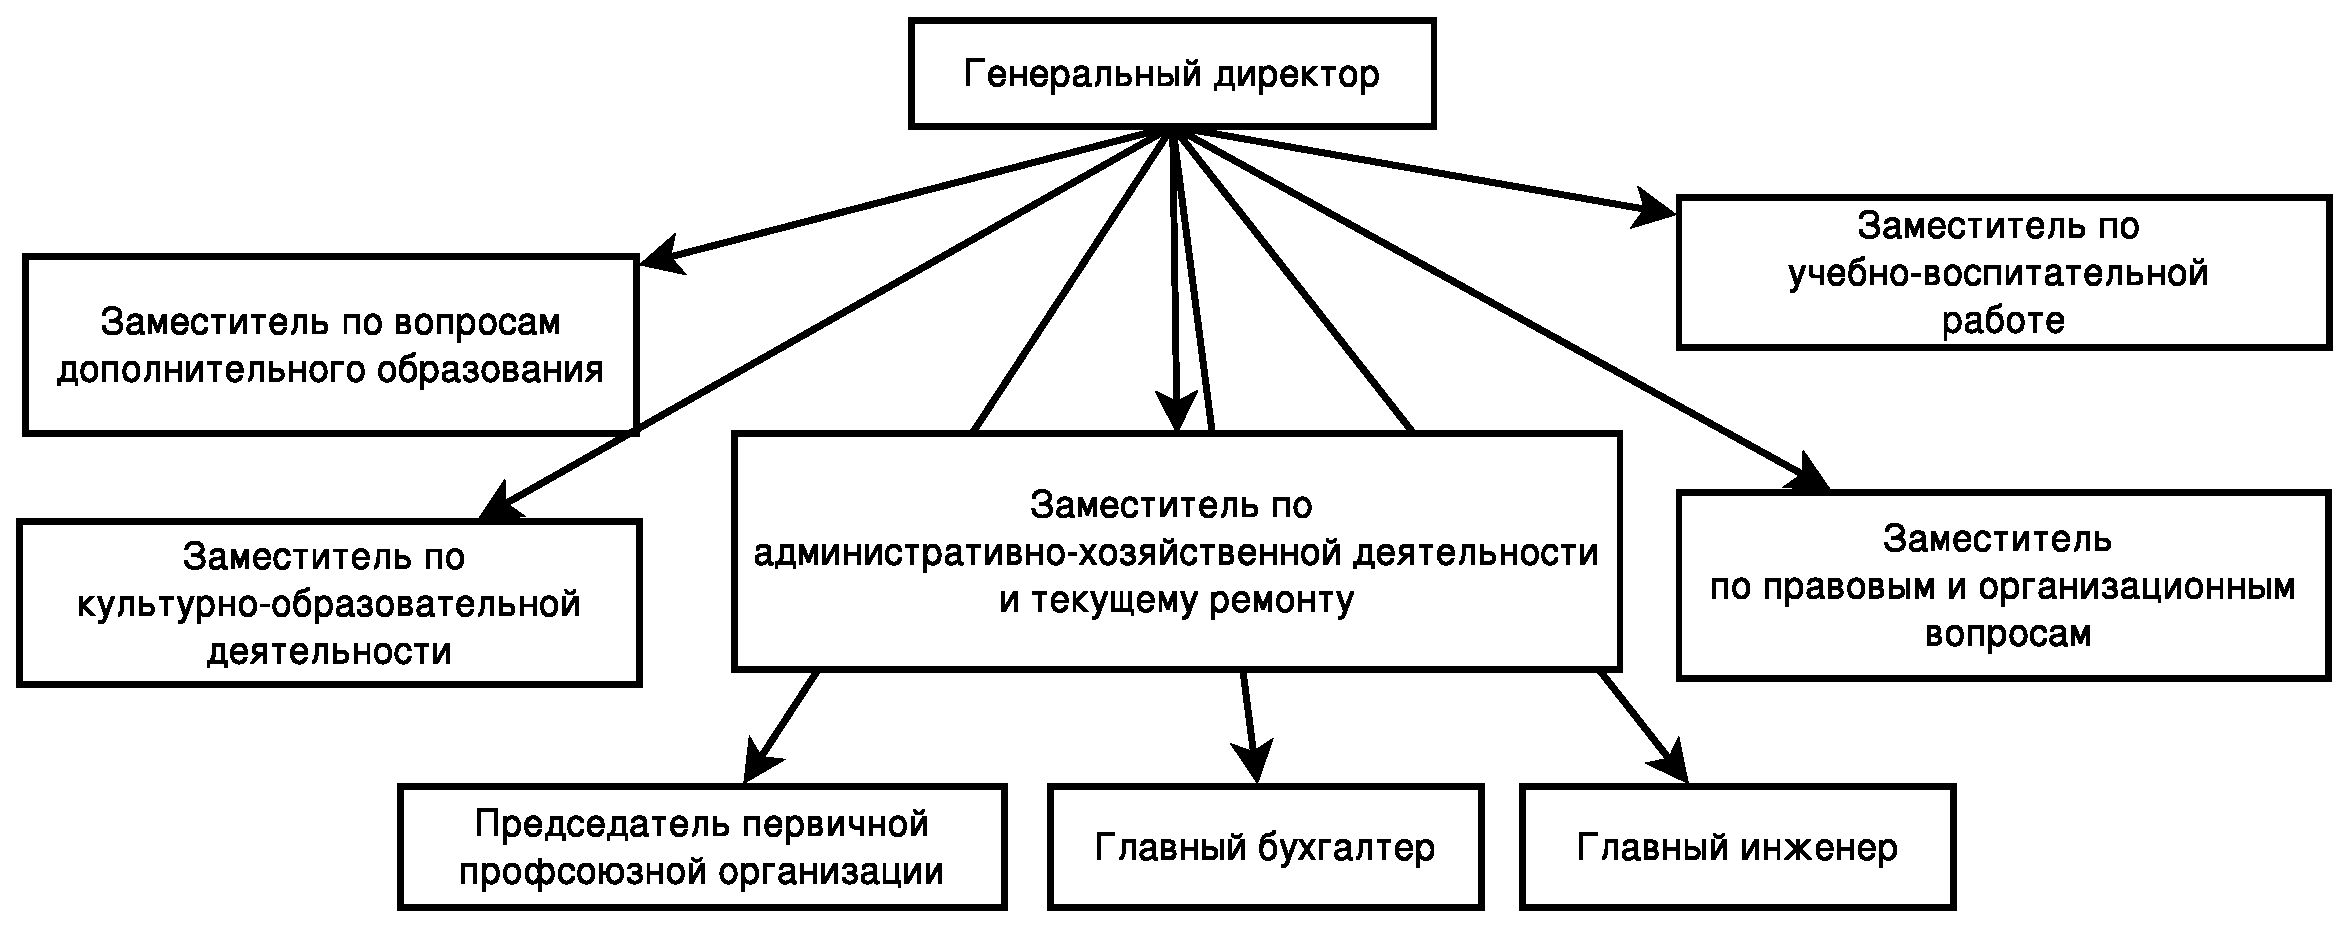
\includegraphics[height=160mm, width=0.8\textwidth, clip, keepaspectratio]{management_structure.eps}
   \caption{Структура управления организацией}\label{fig:fig_management_struct}
 \end{figure}

Сотрудники дворца разделены на коллективы или отделы, отвечающие за определенный вид деятельности. 
Каждый отдел в свою очередь имеет большое количество своих подразделений. У каждого коллектива или отдела есть свой директор, один или несколько заместителей и большое количество сотрудников.

Основной функцией дворца является оказание образовательных и воспитательных услуг, предоставление которых оказывают учебные коллективы, осуществляющие свою деятельность под управлением методических подразделений самого Дворца
и управляющих организаций МОиН города. Кроме непосредственно обучения сотрудники  составляют различные учебные программы, рабочие планы, отчеты, разрабатывают учебно-методические пособия.
Обеспечением текущей деятельности дворца, в аспекте поддержания в надлежащем состоянии оборудования, коммуникаций занимаются сервисные подразделения Дворца. Схема должностей СПБГТЮ представлена на рисунке 
\ref{fig:fig_management_struct}.

\subsection{Задачи требующие инфраструктурного сопровождения}
Рассмотрим подробнее работу сервисных сотрудников на примере реализации слоевого разделения ИТ- инфраструктуры, которое было описано ранее.

\begin{table}[ht]
  \centering %центрируем таблицу
  \caption{Слои инфраструктуры}\label{tab:tab1}
\begin{tabular}{|c|p{130mm}|}
\hline Слой & Описание \\ 
\hline Пользовательский & Во дворце на данном этапе формировнвания ИТ-инфраструктуры компьютеры полностью находятся в распоряжении пользователей  (сотрудников, учащихся), за исключением их первоначальной установки, которая обеспечивается сотрудниками отдела информационных технологий и компьютерного обеспечения (ОИТКО). \\ 
\hline Функциональный & Можно выделить следующие объекты:
информационные услуги (виртуальные машины, СПС), 
люди, предоставляющие эти услуги
Предоставляются ОИТКО. \\ 
\hline Информационный & Процесс управления и обмена информацией с помощью серверов (почта, FTP  т.д.). Регламент разрабатывается в подразделении ОИТКО. \\ 
\hline Коммуникационный & Локальная сеть. Все подключения имеют единую центральную точку. \\ 
\hline 
\end{tabular} 
\end{table}
\subsection{Ограничения накладываемые на информационное сопровождение}
\subsection{Предположительные архитектурные решения и задачи информационной системы}

\section{Обзор аналогов}
\subsection{Samba}

Samba - серверное ПО реализующее протоколы CIFS, SMB для доступа к сетевым ресурсам. 
Минусом данного варианта реализации является ориентированность на работу в локальной сети, 
отсутствие версионирования файлов(реализуется только с помощью версионных ФС, реализации 
которых в Linux не достаточно протестированы для применения в промышленной эксплуатации).

\subsection{FTP с разделением прав}

Данное решение сложно в настройке, использовании. У этого решения отсутствует возможность 
<<прозрачной>> работы с файлами. Файлы требуется сначала загрузить на локальный диск, внести 
изменения и после этого загрузить обратно на сервер. При этом не сохраняется предыдущая версия 
файла. При использовании такого решения, сложно получать информацию об изменениях~в правах, 
модификациях файлов и дерева каталогов. Версионность реализуется с только с помощью версионных ФС.

\subsection{Системы контроля версий}

Системы контроля версий такие как: git, svn, cvs; 
требуют определённой подготовки от пользователя. Это решение требует от пользователя ручного 
помещения данных в хранилище. Невозможно ограничить глубину сохранения версий файлов.

\section{Формализация техического задания}
\subsection{Платформы}
\subsection{Средства}
\subsection{Функциональные ограничения}


\chapter{Глава 2. Проектирование}
\section{Системные архитектурные решения}
\subsection{Распределение задач между компонентами}
\subsection{Описание задач решаемых отдельными компонентами}
\subsection{Описание интерфейсов между компонентами}

\section{Архитектура программы}
\subsection{Архитектура БД}
\subsection{Архитектура клиентской части}
\subsection{Архитектура сервера приложений}
\section{Проектирование инфраструктуры}
\subsection{Оценка требований к серверу}
\subsection{Оценка требований к рабочему месту пользователя}
\subsection{Оценка требований к пропускной способности канала}

\chapter{Глава 3. Реализация}
\section{Особенности реализации БД}
\section{Особенности реализации инструмента администрирования}
\section{Особенности реализации клиентской части}
\section{Особенности тестирования и отладки}
\section{План внедрения и отладки}
\subsection{Организационные мероприятия}
\subsection{Технические мероприятия}
\subsection{Мероприятия сопровождения}
\section{Требования}

\subsection{Основные требования}
В проекте используются только компоненты распространяющиеся под свободными лицензиями. 
Решение должно функционировать в операционной системе GNU/Linux.

Решение должно предоставлять пользователям защищённый сетевой доступ к 
хранилищу данных с разграничением прав доступа на создание, модификацию, удаление 
файлов и каталогов.

Требуется ведение журнала активности пользователей, включающего в себя информацию о следующих действиях: 

\begin{itemize}
\item дату и время входа/выхода пользователя
\item создание файла
\item модификация файла
\item удаление файла
\item установка блокировки на файл
\item снятие блокировки с файла
\end{itemize}

Клиентская часть предоставляет удобный доступ пользователя к файлам и директориям, на которые ему были 
установлены права доступа такие как: чтение, запись, удаление файлов и каталогов.
Требуется разработать инструмент позволяющий:

\begin{itemize}
\item получать информацию об изменениях произошедших с последнего входа пользователя в систему	
\item выполнять аутентификацию пользователя по логину/паролю	
\item выполнять подключение рабочей области пользователя в дерево каталогов
\end{itemize}

\subsection{Описание ролей в системе}

Необходимо осуществлять разделение пользователей по следующим ролям:
\begin{itemize}
\item Пользователь в соответствие со своими правами имеет доступ к 
файлам и каталогам подразделения и к общим каталогам. Имеет доступ к 
предыдущим версиям своих файлов на чтение. 
\item Администратор подразделения может назначать права доступа для сотрудников 
подразделения, создавать и удалять каталоги в каталоге подразделения. 
Имеет доступ на чтение к предыдущим версиям файлов подразделения	
\item Администратор создает и удаляет учётные записи пользователей, 
записи подразделений, назначает права доступа, имеет полный
доступ к дереву каталогов, имеет полный доступ к предыдущим версиям файлов.
\end{itemize}

\chapter{Архитектура}
Предлагается трёхзвенная архитектура: Клиент -- сервер приложений -- хранилище данных.

Задачей хранилища данных является хранение файлов пользователей, дерева каталогов, 
информации о пользователях и их правах доступа. Бизнес логика реализуется на сервере 
приложений. В рамках которой обеспечивается: 

\begin{itemize}
\item авторизация пользователей,
\item предоставление требуемых файлов и каталогов для работы в 
соответствие с правами доступа, 
\item блокировка используемых файлов и получение обновлённой 
версии с возможным сохранением предыдущих версий файла.
\end{itemize}
\chapter{Реализация}
\chapter{Экономическая часть}
\chapter{Безопасность}

\Conclusion
заключение


\end{document}